\documentclass[11pt]{article}
\usepackage{graphicx}
\usepackage[top=0.75in, bottom=1.75in, left=1in, right=1in,includefoot]
{geometry}
\usepackage{fancyhdr}
\usepackage[english]{babel}
\usepackage[math]{blindtext}
\usepackage{listings}
\usepackage{xcolor}
\usepackage{float}
\usepackage{amsmath}
\usepackage{amssymb}
\usepackage{mathpartir}
\usepackage{hyperref}
\usepackage{cleveref}
\usepackage{stmaryrd}
\usepackage[OT1]{fontenc}
\usepackage{utilities}
\usepackage{relsize}


\providecommand{\todo}[1]{\textcolor{red}{\textbf{TODO:} #1}}
\makeatletter
\@addtoreset{figure}{section}
\makeatother
\renewcommand{\thefigure}{\thesection.\arabic{figure}}
\newcommand{\List}{\mathsf{List}}
\newcommand{\LDispose}{\mathsf{LDispose}}
\newcommand{\LLen}{\mathsf{LLen}}
\newcommand{\CClist}{\mathsf{CClist}}
\newcommand{\CCllist}{\mathsf{CCllist}}
\newcommand{\addnode}{\mathsf{addnode}}
\newcommand{\reach}{\mathsf{reach}}
\newcommand{\Assert}{\mathsf{Assert}}
\newcommand{\True}{\mathsf{True}}
\newcommand{\False}{\mathsf{False}}
\newcommand{\Emp}{\mathsf{emp}}
\newcommand{\sepimp}{\mathrel{-\mkern-6mu\ast}}
\newcommand{\Eval}[1]{\mathcal{E}[\![#1]\!]_{e,s}}
\newcommand{\Val}{\mathsf{Val}}
\newcommand{\Heap}{\mathsf{Heap}}
\newcommand{\Pred}{\mathsf{pred}}
\newcommand{\pv}{\mathsf{pv}}
\newcommand{\Mod}{\mathsf{mod}}
\newcommand{\Bool}{\mathsf{Bool}}
\newcommand{\Var}{\mathsf{Var}}
\newcommand{\Exp}{\mathsf{Exp}}
\newcommand{\Null}{\mathsf{null}}
\newcommand{\blueassn}[1]{\textcolor{blue}{#1}}
\newcommand{\triple}[3]{\vdash\ \blueassn{\{#1\}}\ #2\ \blueassn{\{#3\}}}
\newcommand*{\defeq}{\mathrel{\vcenter{\baselineskip0.5ex \lineskiplimit0pt
                     \hbox{\scriptsize.}\hbox{\scriptsize.}}}%
                     =}
\newcommand*{\ddefeq}{\mathrel{\vcenter{\baselineskip0.5ex \lineskiplimit0pt
                     \hbox{\scriptsize.}\hbox{\scriptsize.}}}%
                      \mathrel{\vcenter{\baselineskip0.5ex \lineskiplimit0pt
                     \hbox{\scriptsize.}\hbox{\scriptsize.}}}
                     =\ }


\pagestyle{fancy}
\fancyhead[L]{\fancyhdrbox[c]{\Large \slshape \sffamily 
Separation Logic and Compositional Symbolic Execution:\\
Verification and Bug Detection at Scale}}
\fancyhead[C]{}
\fancyhead[R]{\large \sffamily \bfseries Philippa Gardner}
\fancyfoot[L]{\fancyhdrbox[b]{\sffamily \small Compiled By: \\ 
\normalsize \sffamily Dinghong Zhong, Samuel Dodson, Daniel Pinto}}
\fancyfoot[C]{\thepage}
\fancyfoot[R]{\fancyhdrbox[b]{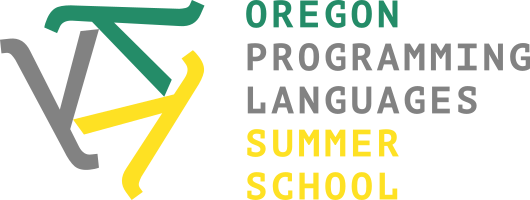
\includegraphics[width=1in]{oplssLogo.png}}}
\renewcommand{\footrulewidth}{0.5pt}

\fancypagestyle{plain}{
\fancyhf{}
\fancyfoot[L]{\fancyhdrbox[b]{\sffamily \small Compiled By: \\ 
Dinghong Zhong, Samuel Dodson, Daniel Andres Pinto Alvarado}}
}

\setlength{\parindent}{0pt}
\setlength{\parskip}{2ex}
\setlength{\headheight}{1.25in}
\setlength{\footskip}{32pt}
\begin{document}

\thispagestyle{plain}
\begin{center}
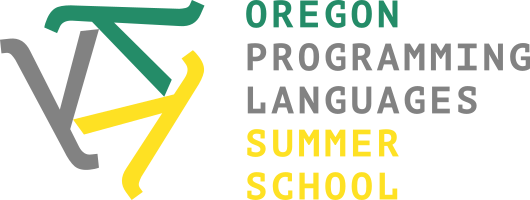
\includegraphics[width=3in]{oplssLogo.png}\\
\sffamily \LARGE \slshape 
Separation Logic and Compositional Symbolic Execution:\\
Verification and Bug Detection at Scale\\[2ex]
\upshape Philippa Gardner\\[2ex]
\large Lecture 2 - \slshape June 25, 2026
\end{center}

These are the notes for the second lecture of the OPLSS 2026 course on Separation
Logic and Compositional Symbolic Execution, taught by Philippa Gardner. 
The official lecture slides are available at \url{https://gillianplatform.github.io/docs/oplss26/Lecture2.pdf}.

\section{Describing Structures Beyond Classic Linked Lists}

The lecture gives the following add-node example for Collections-C singly linked lists:

\[
\hoareT{x = x \star v = v \star \CClist(x,\alpha)}
        {\CCllist\ \addnode(x,v)}
        {\CClist(ret,\alpha \cdot [v])}
\]

\begin{lstlisting}[basicstyle=\ttfamily\small,columns=fullflexible]
CCllist addnode(x, v) {
   n := new(2);
   [n] := v;
   l := [x];
   if (l = 0) {
      [x] := l + 1; [x + 1] := n; [x + 2] := n
   } else {
      t := [x + 2];
      [t + 1] := n; [x + 2] := n; [x] := l + 1
   };
   return x
}
\end{lstlisting}

The postcondition states that the returned Collections-C list contains the original sequence $\alpha$ extended by the singleton list $[v]$.

Separation logic also allows us to describe complex structures, such as N-ary trees:

\begin{alignat*}{3}
tree(x,c) &\quad \on{def}{=}\quad && (x \mapsto 0,\_ \star c = 1)\\
&\quad \quad && \vee \left(\exists\   n > 1, \vec{p}, \vec{c}. x \mapsto n \star c = \sum_{i = 1}^n c_i \star P(n,c) \right)\\
P(n,c) &\quad = \quad &&  \bigcircledast_{1 \leq i \leq n} (x+i \mapsto p_i \star tree(p_i,c_i) \wedge 1 \leq c_i < c)
\end{alignat*}

The predicate $tree(x,c)$ describes a tree $x$ with $c$ total cells used by either constructing a leaf with value $0$ (and an empty box for uniformity), or by establishing what the head $x$ is pointing to, and ensuring we have enough space for each of the children ($c_i$) and describing them recursively.


An example of an N-ary Tree described by the specification is the one portrayed in Figure \ref{fig:ntree}

\begin{figure}[H]
\centering
\begin{tikzpicture}[
  cellnode/.style={draw, minimum width=0.8cm, minimum height=0.7cm,
                   anchor=center, inner sep=0pt, font=\large},
  >=Stealth
]
 
% Root node (3 cells): value | left pointer | right pointer
\matrix (root) [matrix of nodes, nodes={cellnode},
                column sep=-\pgflinewidth, row sep=0pt]
  at (0,0) {2 & $\bullet$ & $\bullet$ \\};
 
% Left child of root (3 cells)
\matrix (left) [matrix of nodes, nodes={cellnode},
                column sep=-\pgflinewidth, row sep=0pt]
  at (-3,-3) {2 & $\bullet$ & $\bullet$ \\};
 
% Right child of root (2 cells: leaf)
\matrix (right) [matrix of nodes, nodes={cellnode},
                 column sep=-\pgflinewidth, row sep=0pt]
  at (3,-3) {0 & $-$ \\};
 
% Leaves under "left"
\matrix (leaf1) [matrix of nodes, nodes={cellnode},
                 column sep=-\pgflinewidth, row sep=0pt]
  at (-4.5,-6) {0 & $-$ \\};
 
\matrix (leaf2) [matrix of nodes, nodes={cellnode},
                 column sep=-\pgflinewidth, row sep=0pt]
  at (-1.5,-6) {0 & $-$ \\};
 
% Incoming arrow labeled E_x
\node (Ex) at (-0.4,1.7) {$E_x$};
\draw[->] (Ex.south) -- (root-1-1.north east);
 
% Root's two pointers
\draw[->] (root-1-2.south) to[out=-90, in=90] (left-1-1.north);
\draw[->] (root-1-3.south) to[out=-90, in=90] (right-1-1.north);
 
% Left child's two pointers
\draw[->] (left-1-2.south) to[out=-90, in=90] (leaf1-1-1.north);
\draw[->] (left-1-3.south) to[out=-90, in=90] (leaf2-1-1.north);
 
\end{tikzpicture}
\caption{N-ary Tree}
\label{fig:ntree}
\end{figure}

Following the same schema, we could also define Hash Tables, Doubly Linked Lists, Collections-C linked lists, $\dots$

\section{Formalizing Proof Sketches}

In the previous lecture we saw how we could describe informally the behaviour of a program, such as \verb!LLen! (which computed the length of a linked list recursively) via Hoare triples with preconditions and postconditions encoded in separation logic. But how can we reason about the program in a formal way?

For that, we'll use the proof rules defined in Figure \ref{fig:proof_rules} (\textbf{\textcolor{red}{frame}}, \textbfr{cons}equence, \textbfr{exist}ential elimination, and \textbfr{seq}uencing) to do proof derivations.

\begin{figure}[H]
\[
\begin{prooftree}
\hypo{\vdash \hoareT{P}{C}{Q}}
\hypo{\Mod(C) \cap fv(R) = \emptyset}
\infer2[frame]{\vdash \hoareT{P \star R}{C}{Q \star R}}
\end{prooftree}
\qquad 
\begin{prooftree}
\hypo{\models P \Rightarrow P'}
\hypo{\vdash \hoareT{P'}{C}{Q'}}
\hypo{\models Q' \Rightarrow Q}
\infer3[cons]{\vdash \hoareT{P}{C}{Q}}
\end{prooftree}
\]
\[
\begin{prooftree}
\hypo{\vdash \hoareT{P}{C}{Q}}
\infer1[exists]{\vdash \hoareT{\exists x. P}{C}{\exists x. Q}}
\end{prooftree}
\quad
\begin{prooftree}
\hypo{\vdash \hoareT{P}{C_1}{Q}}
\hypo{\vdash \hoareT{Q}{C_2}{R}}
\infer2[seq]{\vdash \hoareT{P}{C_1;C_2}{R}}
\end{prooftree}
\]
\label{fig:proof_rules}
\caption{Proof rules for reasoning about Hoare triples}
\end{figure}

\textbfr{Notation}: $\Mod : C \rightarrow \Var$ is a function which maps commands to the (program) variables which are (possibly) modified, while $fv$ returns the set of free variables (program or logical) from an assertion expression.
In particular, $x$ is modified by assignments such as $x := E$, $x := [E]$, $x := new(E)$, and $x := f(\vec{E})$, but not by mutation commands such as $[E] := E$.
Recall that the proof rules are sound: $\vdash \{P\}C\{Q\} \Rightarrow \models \{P\}C\{Q\}$.


Let's consider the example of the previous lecture, in particular:

\begin{ntabular}{l}
\crlf \} else \{\\
\crlf \tab \assert{$\text{x}=x \star list(x,\alpha)\star n,t = null \star x \not = null$}\\
\crlf \tab \comment{unfold list predicate to recursive case, identify the resource needed}\\
\crlf \tab \assert{$\exists v,\beta, y. x \mapsto v, y \star \alpha = v : \beta \star list(y,\beta) \star n,t=null$}\\
\crlf \tab \commentBlock{exists,frame+cons}{
\begin{ntabular}[5]{l}
	\crlf \assert{$x \mapsto v,y \star list(y,\beta) \star n,t=null$}\\
	\crlf t := [x + 1];\\
	\crlf \comment{Use the fcall rule to consume precondition and produce postcondition}\\
	\crlf \assert{$x \mapsto v,y \star list(y,\beta) \star n=null \star t = y$}\\
	\crlf n := llen(t);\\
	\crlf \assert{$x \mapsto v,y \star list(y,\beta) \star n = |\beta |$}\\
	\crlf n := n + 1;\\
	\crlf \assert{$x \mapsto v, y \star list(y,\beta) \star n = |\beta | + 1$}
\end{ntabular}
}\\
\crlf \tab \comment{frame back assertions, add exists and fold back list predicate}\\
\crlf \tab \assert{$\exists v,\beta, y. x \mapsto v, y \star \alpha = v:\beta \star list(y,\beta) \star n = |\beta | + 1$}\\
\crlf \tab \assert{$list(x,\alpha) \star n = |\alpha |$}\\
\crlf \}
\end{ntabular}
 
Let's use proof rules to verify the else body after unfolding the list predicate.

\begin{figure}[H]
\[
\begin{prooftree}
\hypo{\dots}
\infer1[\textbf{1}]{\Gamma \entails \hoareT{P}{t := [x+1]}{S}}
\hypo{\dots}
\infer1[\textbf{2}]{\Gamma \entails \hoareT{S}{n := llen(t)}{R}}
\infer2[seq]{\Gamma \entails \hoareT{P}{t := [x+1] ; n := llen(t)}{R}}
\hypo{\dots}
\infer1[]{\Gamma \entails \hoareT{R}{n := n + 1}{Q}}
\infer2[seq]{\Gamma \entails \hoareT{P}{t := [x+1] ; n := llen(t); n := n+1}{Q}}
\infer1[exists $\times$ 3]{\Gamma \entails \hoareT{\exists v,\beta,y. P}{t := [x+1] ; n := llen(t); n := n+1}{\exists v,\beta,y. Q}}
\end{prooftree}
\]
\label{fig:llen_innerB}
\caption{Proof for LLen inner block}
\end{figure}

If we allow $P,S,R,Q$ to stand for:

\begin{itemize}
	\item $P=x \mapsto v,y \star \alpha = v : \beta \star list(y,\beta) \star n,t=null$
	\item $S = x \mapsto v,y \star \alpha = v:\beta \star list(y,\beta) \star n=null \star t=y$
	\item $R = x \mapsto v, y \star \alpha = v : \beta \star list(y,\beta) \star n = | \beta |$
	\item $Q = x \mapsto v, y \star \alpha = v : \beta \star list(y,\beta) \star n = | \beta | + 1$
\end{itemize}

The two remaining subderivations used in Figure \ref{fig:llen_innerB} are:

\begin{figure}[H]
\small
\[
\begin{prooftree}
\hypo{x \notin \pv(\Null)}
\infer1[lookup]{\Gamma \entails \hoareT{t = \Null \star x + 1 \mapsto y}{t := [x+1]}{t = y \star x + 1 \mapsto y}}
\infer1[frame]{\Gamma \entails \hoareT{t = \Null \star x + 1 \mapsto y \star F}{t := [x+1]}{t = y \star x + 1 \mapsto y \star F}}
\infer1[cons]{\Gamma \entails \hoareT{P}{t := [x+1]}{S}}
\end{prooftree}
\]
\[
F = x \mapsto v \star \alpha = v:\beta \star list(y,\beta) \star n = \Null
\]
\caption{LLen proof derivation, recursive case 1}
\end{figure}

\begin{figure}[H]
\small
\[
\begin{prooftree}
\hypo{\hoareT{x = x \star list(x,\alpha)}{\LLen(x)}{list(x,\alpha) \star ret = |\alpha|} \in \Gamma}
\infer1[fcall]{\Gamma \entails \hoareT{y \in \Val \star t = y \star list(y,\beta)}{n := llen(t)}{list(y,\beta) \star n = |\beta|}}
\infer1[frame]{\Gamma \entails \hoareT{y \in \Val \star t = y \star list(y,\beta) \star F}{n := llen(t)}{list(y,\beta) \star n = |\beta| \star F}}
\infer1[cons]{\Gamma \entails \hoareT{S}{n := llen(t)}{R}}
\end{prooftree}
\]
\[
F = x \mapsto v,y \star \alpha = v:\beta
\]
\caption{LLen proof derivation, recursive case 2}
\end{figure}

Then we can see most of the work is just either joining commands naturally via the \textbfr{seq} rule, or unfolding definitions so we can meet the precondition of a function call, as can be seen by the $S$ condition.

\section{Compositional Symbolic Execution}

The second half of the lecture explains how tools bridge the gap between proof sketches and automated reasoning. Compositional symbolic execution symbolically executes a partial symbolic state, uses \emph{produce} to assume the resources described by a precondition, and uses \emph{consume} to check that the resources required by a command or a postcondition are available. First-order path constraints are checked by SMT solvers such as Z3.

The lecture separates the theory and practice of compositional symbolic execution: the theory is tool-independent, parametric in the memory model, and supports both compositional verification and true bug detection, while Gillian\footnote{Demo video: \url{https://www.youtube.com/watch?v=5TTBX4ecZkk}.} is the maintained platform implementation.

The symbolic state used in Gillian has four parts:
\[
\hat{\sigma} = (\hat{s}, \hat{\mu}, \widehat{\Pred}, \hat{\pi})
\]
where $\hat{s} : \mathsf{PVar} \rightharpoonup_{\mathrm{fin}} \mathsf{LExp}$ is the symbolic store, $\hat{\mu} : \mathsf{LExp} \rightharpoonup_{\mathrm{fin}} \mathsf{LExp}$ is the symbolic linear heap, $\widehat{\Pred}$ stores user-defined predicate instances, and $\hat{\pi}$ is the symbolic path condition.

For the recursive case of $\LLen$, compositional symbolic execution follows the same logical structure as the proof sketch:
\begin{enumerate}
	\item produce the initial symbolic state from the precondition $x = x \star list(x,\alpha)$;
	\item split on $x = \Null$;
	\item in the non-null branch, unfold $list(x,\alpha)$ to obtain $x \mapsto v,y \star list(y,\beta) \star \alpha = v:\beta$;
	\item execute the lookup $t := [x+1]$ and update the symbolic store with $t = y$;
	\item for $n := \LLen(t)$, consume the callee precondition for $t$ and produce its postcondition;
	\item execute $n := n+1$, fold the list predicate back, and consume the final postcondition.
\end{enumerate}

\end{document}
